\documentclass[a4paper,11pt,pdftex,halfparskip,cleardoubleempty]{scrbook}
\usepackage{wrapfig}
\usepackage[pdftex]{graphicx}
\usepackage{eso-pic}
\usepackage{fixltx2e}
\usepackage{subfig}

% bibloiography
\usepackage{listings}

%table positioning
\usepackage{float}
\restylefloat{table}

%because of my name
%\usepackage[slovak]{babel}
%\usepackage[utf8]{inputenc}

\graphicspath{
 {img/}
 {img/CrossCorelation/Releases/}
 }
\newcommand*{\xchapter}{\stepcounter{chapter}\setcounter{section}{0}\addchap}
\renewcommand*{\thesection}{\arabic{section}}

% define medatata
\def\MTitle{The Title}
\def\MAuthor{Martin Ďurček}
\def\MKeywords{Keyword 1 \sep Keyword 2\sep Keyword 3\sep Keyword 4}
\def\MOrg{Universit{\"a}t Innsbruck}
\def\MDate{\today}
\def\MInstitution{Department of Computer Science}
\def\MSupervisor{Ass.-Prof. Dr. Michael Felderer}
\def\MGroup{Research Group Quality Engineering}

 
\begin{document}

\pagestyle{empty}


\begin{titlepage}
\rule{0mm}{1mm}
\vspace*{10mm}
\begin{wrapfigure}{l}{3.25cm}
    
\includegraphics[width=3cm]{uni-logo-4c_new}
\end{wrapfigure}
\begin{flushright}
    \setlength{\unitlength}{1cm}
    {\large \MOrg \vskip 5mm
    \MInstitution}\\
    \textbf{\large \MGroup}
    \vskip 15mm
    \textbf{\Large M\,A\,S\,T\,E\,R\,\,\,T\,H\,E\,S\,I\,S}
\end{flushright}

\begin{center}
    \vskip 25mm
    {\LARGE\bf \MTitle}
    \vskip 5mm
    \vskip 1cm
    {\large \textbf{\MAuthor}}\vskip 15mm
    \vskip 2cm
    {\large Supervisor: Prof. Dr. Michael Felderer}
    \vfill
    {\large Innsbruck, 10. October 2018} 
\end{center}
\AddToShipoutPicture{
    \put(-55,55){
        \parbox[b]{\paperwidth}{
             \hfill 
\includegraphics[scale=0.35]{UniWatermark}
        }
    }
}
\end{titlepage} 

\ClearShipoutPicture

\cleardoublepage
\tableofcontents 
\cleardoublepage
\pagenumbering{arabic}
\pagestyle{plain} 

\chapter{Introduction}
\label{chp:introduction}
 
 
\chapter{Proposed framework}
\label{chp:proposedFramework}
Despite Open-Source Software being popular, widely used and implemented in production, there's no definite consent regarding the ideal and most favoured release frequency and size. Some projects release several times per month while the others only once per quarter or even less. Also releases differ in size, number of commits and fixed issues they address. My goal is to explore some potential hidden patterns which could be generalized and used in the future release planning and policy in Open-Source space.\\
Another issue and not only with Open-Source projects are bugs and finding workarounds and temporary solutions for them. We all know the scenario when a correct code doesn't function properly. We head to Stack Overflow or Reddit and start to look for similar problems. If lucky enough, we find a question with a solution presented in the comment section. But that's not always the case. Especially questions about faults caused by library/framework bugs have often empty and not really helpful comment sections because there should not be such problem in the first place. Such situations can eat up a lot of developers' time and kill productivity. Therefore I hoped to create an algorithm which could link corresponding GitHub and Stack Overflow items and make these frustrating situations easier.

This thesis is divided into 2 parts. I aimed to create a framework which could be potentially used as a base of tool used to recognize level of user satisfaction and its sudden changes. Second part of the framework should be able to find and link pairs of issues reported in bug tracking systems and their respective social media entries. Both parts of the framework use various text processing methods, sentiment analysis concentrating more on machine learning while bug linking utilizes topic modelling and text similarity concepts.\\
\begin{figure}%
    \centering
	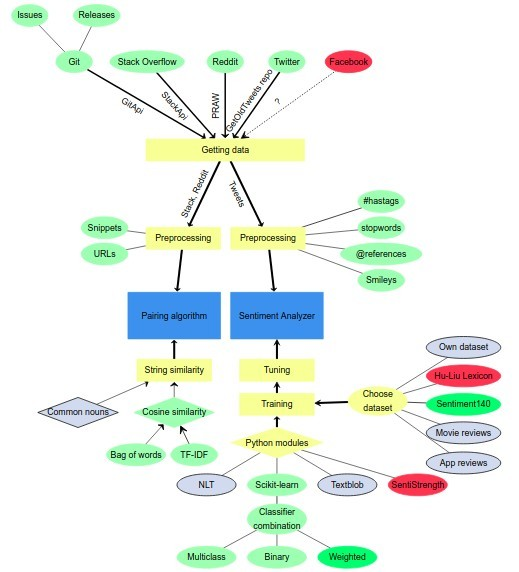
\includegraphics[width=15cm]{dataflow_final_yed.jpg}
    \caption{Brief sketch of dataflow in the proposed framework}%
    \label{fig:frameworkDataflow}%
\end{figure}
As can be seen in Figure \ref{fig:frameworkDataflow}, two final products of the framework are sentiment classifier and linking algorithm. Green elements are the ones used in final solution, grey ones were tested and considered and red ones were left out or not possible to implement. Work on the framework could be divided into several steps:
\begin{enumerate}
\item{\textbf{Getting the data} - there is no data science, machine learning or natural language processing without the data. That is why the very first step is to create a mechanism to easily mine data from various sources. Git mining is required to get information about OSS projects and is described in subsections number \ref{ssec:gitReleaseDatesMining} and \ref{ssec:issuesMining} while Twitter, Reddit and SO were mined to provide data which are the target of analysis \ref{ssec:GettingData}.}
\item{\textbf{Data preprocessing} - all textual information, especially those which originate on social media contain noise. To get rid of all this extra information, which might cause inaccuracies and faults, data preprocessing is a necessary step.}
\item{\textbf{Finding a right training dataset} - since the performance of any ML algorithm is very tightly bound to the training data used, this step should not be neglected and be considered as important step as any other. It is described in the Section \ref{sec:trainingDatasets}.}
\item{\textbf{Choosing a tool/module/library and particular classification algorithm} - there are many algorithms used for classification but environment for their usage and best performance differs greatly. To choose a correct algorithm and find the best combination of parameter values is often a long process. Things do not get any easier when we take into account that there are not only many algorithms but they are actually also implemented in several programming languages and libraries. Inconsistencies between results of several SE modules were pointed out by Bin Li at al. in his paper \textit{How far can we go}. My approach to problems and challenges of this step are described in great detail in sections number \ref{sec:languageProcessingTools} and \ref{sec:classifierEvaluation}}
\item{\textbf{Topic modeling and text similarity} - this is the crucial step for the second part of the framework. Once the data are downloaded from Git as well as from social media, the last step to do is to find the matches.   This part is described in Chapter \ref{chap:pairingBugs}.}
\end{enumerate}
After all the steps are implemented, proposed framework will be completed. But that does not guarantee that the output data are easy to interpret. That's why one extra additional step is needed. Using some statistics and data science methods, I am interpreting the results in Subsection \ref{ssec:crossCorrelation} and Subsection \ref{ssec:crossCorrelationCommits}.

\newpage
\textbf{This framework targets following research questions:}
\begin{itemize}
\item{\textbf{$RQ_{1}$}: Do the OSS projects which release more often get general better sentiment score on social media?}
\item{\textbf{$RQ_{2}$}: Does a release have an immediate effect on sentiment?}
\item{\textbf{$RQ_{3}$}: Is there a correlation between sentiment change and size of the release (number of commits) ?}
\item{\textbf{$RQ_{4}$}: Is it possible to link social media entries to their respective bugs which they talk about?}
\end{itemize}



\chapter{Social Media}
\label{chp:socialMedia}
Social media is a term referring to online communication channels meant for social interaction, content-sharing and collaboration. Over time, this term became widely used, its exact definition somewhat blurred and if really wanted, most of the today's websites could be labeled as social media. In context of this thesis,  I refer to social media in its “original” meaning. To be considered a social media platform, most of following features usually need to be fulfilled:

\begin{itemize}
  \item \textbf{User accounts} - platform allows users to create and run their own accounts that they can log into. These are online representations of their owners and serve as a too to reach and interact with other users.
  \item \textbf{Profile pages} - pages which represent an individual, might it be a real person, group of people or company. It should contain several personal information about the user like bio, profile picture or some other personal data.
  \item \textbf{Friends, followers, groups} - list of accounts whose owners have some form of a relationship  or common interest with the user.
  \item \textbf{News feeds} - Area where all new content from other connected entities appears.
\end{itemize}

Even if a platform fulfills these requirements, it doesn't necessarily have to be classified as social networking platform as pointed out in Haewoon Kwak's paper\cite{kwak2010twitter}.

\section{Potential of social media data mining}
Social media are changing the way that information is passed across societies and around the world.\cite{mayfield2008social}
Among many other potentials of social media, there is a huge amount of data generated on daily basis. These data carry lots of real world data and if used correctly, can offer deep insight into almost any area. The process of analyzing these data and searching for repetitive reoccurring patterns with goal of predicting future trends is also called social media mining. Successful mining can not only save money and time spent on getting the data in more traditional way like surveys but can also provide crucial factor in planning or decision making of businesses. Although internet is one big hole and contains lot of false facts and desinformation, there is indication that social networks tend to favour
valid information over rumours.\cite{castillo2011information} 

\section{Data}
\subsection{Getting data} \label{ssec:GettingData}
As you will have a chance to see, big social networking platforms started realizing that data they own are a “golden egg” and getting raw full data from them got much more difficult than it was in the early years of social media age.

\paragraph{Twitter:}
When talking about sentiment analysis of social media, analysis of Twitter data has in last couple of years became almost a default choice. This change can be nicely seen in the Mantyla, Graziotin and Kuutila's \cite{mantyla2018evolution} wordcloud of SE papers before and after 2013.\ref{fig:papersWordcloudHistory}.

\begin{figure}[H]%
    \centering
	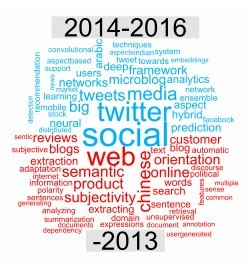
\includegraphics[width=8cm]{papersWordcloudHistory.jpg}
    \caption{Wordcloud comparison of pre and post 2013 SE papers \ref{fig:papersWordcloudHistory}}%
    \label{fig:papersWordcloudHistory}%
\end{figure}

To get the data from Twitter,  I first tried to use the Twitter API but I very early got to know that Twitter is well aware of the worth of their data. They don't provide tweets older than 2 weeks what basically made their API inapplicable for my purposes. The only way how to get historical Twitter data is actually:

\begin{itemize}
  \item collect them over time
  \item buy them from Twitter
  \item buy them from other companies who collect Twitter dumps over time
\end{itemize}

Therefore to obtain my data, I had to use the Twitter Search Api. To do this I used the project (https://github.com/Jefferson-Henrique/GetOldTweets-python) which provides an extra layer on top of Search Api and simplifies working with it. Using this technique, I managed to get the significant amount of data needed for all my tasks in this thesis.

This repository offers following collection of search parameters which can be used to filter specific tweets according:
\begin{itemize}
  \item setUsername - twitter account without "@"
  \item setSince - lower date bound with format "yyyy-mm-dd"
  \item setUntil - upper date bound with format "yyyy-mm-dd"
  \item setQuerySearch - search text to be matched
  \item setTopTweets - boolean flag whether to return only top tweets
  \item setNear - location are reference 
  \item setWithin - radius from "near" location
  \item setMaxTweets - max amount of tweets to be retrieved
\end{itemize}


I got historical twitter data by looping all projects and their release dates and requested data: 

\begin{itemize}
  \item on the release dates (Listing \ref{lst:onReleaseDatesScript})
  \item in the interval of 2 days before and after  release date (Listing \ref{lst:beforeAfterReleaseDatesScript})
  \item weekly
\end{itemize}


\begin{lstlisting}[caption={Creating command to get Tweets about a project version on release dates},label={lst:onReleaseDatesScript},language=Python]
miningConsoleCommand = "python Exporter.py --querysearch '" + frameworkName + " AND " + version + "' --since " + str(releaseDate) + " --until " + str(afterRelease) + " --output='" + frameworkName + "_" + str(releaseDate) + ".csv" + "'"
\end{lstlisting}


\begin{lstlisting}[caption={Creating command to get Tweets about a project version in particular time interval around release date},label={lst:beforeAfterReleaseDatesScript},language=Python]
miningConsoleCommand = "python Exporter.py --querysearch '" + frameworkName + "' --since " + str(fromDate) + " --until " + str(toDate)  + " --lang " + "en" + " --maxtweets " + str(TWEETS_PER_RELEASE) + " --output='" + frameworkName + ".csv" + "'"
\end{lstlisting}


\paragraph{Facebook:}
I originally planned to use Facebook statuses as a big part of analyzed data. Sadly, this was not possible since Facebook Graph API doesn't allow post searching feature. There was this option till early 2014 with Facebook API 1.x versions but since Graph API has been introduced, there's no way how to make Facebook application send requests to 1.x versions of API. At first, application created before 2014 were still working on top of the early Api versions and it has been maintained but over time, all the applications were migrated to 2.x Api versions. There's currently no public way how to freely get the Facebook posts data. The other types provided by the Api are for example user, page, event, group or place.

\paragraph{Reddit:}
Despite that reddit doesn't offer big amount of user data in OSS projects subreddits, I thought getting and working with Reddit could increase the variety of users and the data which I will be working with. To get the data I used Python Reddit API Wrapper (PRAW) used to directly work with Reddit Api via HTTP requests.

Class Reddit provides a convenient way how to access Reddit API. Instance of this class can be seen as a gateway to interact with API through PRAW. To instantiate this class, user first has to register his application. This gives user unique \textit{useragent} key which identifies the application. This is so that if a program misbehaves for some reason, it can be more easily identified, rather than look like a browser. All mandatory arguments are shown in Listing \ref{lst:redditClassInstance}.

\begin{lstlisting}[caption={Instantiating Reddit class object},label={lst:redditClassInstance},language=Python]
reddit = praw.Reddit(clientid='CLIENTID',clientsecret="CLIENTSECRET", password='PASSWORD',useragent='USERAGENT',username='USERNAME')
\end{lstlisting}

After connection to Api is successful, senting requests with PRAW is straightforward. To get the submissions from a particular subreddit in a specific time interval, just a basic loop shown in Listing \ref{lst:redditSubmissionsLoop} is enough.

\begin{lstlisting}[caption={Getting posts from subreddit},label={lst:redditSubmissionsLoop},language=Python]
for submission in reddit.subreddit(redditName).submissions(FROM, TO)):
\end{lstlisting}

Each post (submission) contains among other information also array-like member variable of all comments. Simply concatenating all those gives the whole textual representation of the discussion.

\textit{*During the writing of this thesis, new Reddit API deprecated the described approach and submission class.}


\paragraph{Stack overflow:}
To extract the questions about the OSS projects of my interest I once again used provided Api. Python module called StackApi offers a way how to communicate with various Stack Exchange Api endpoints - answers, badges, comments, posts, questions, tags and users. To initiate communication with StackAPi, one needs only to specify Stack webpage and choose an endpoint, tag, time interval and if needed also some other non-mandatory parameters. Afterwards, calling \textit{fetch} method starts returning questions. Snippet of how I got the data can be seen in Listing \ref{lst:stacktQuestionsLoop}

\begin{lstlisting}[caption={Getting Stackoverflow questions with StackApi},label={lst:stacktQuestionsLoop},language=Python]
	SITE = StackAPI('stackoverflow')
    	SITE.max_pages = 1;
    	while True:
    		questions = SITE.fetch(
    			'questions',
    			fromdate=date(2012, 5, 8),  # year,month,day
        		todate=date(2016, 4, 15),
        		tagged=project,
        		filter='withbody',
        		sort='creation',
        		page=page
         )
\end{lstlisting}

Stack Exchange is limited on 30 requests per second. Therefore the logic needed to be implemented to avoid a penalization for violating this throttle. At first I intended to use the type “posts” which returns both, questions and answers, but later I've realized how huge amount of data SO contains.  The average count of questions using one of the examined projects names as a tag was around 150 000. Because of this, I had to find out how to filter just the questions with higher probability of talking about bugs. Since the questions on SO do not have any labels which I could use to my advantage like I did with Git issues, I decided to keep just the questions which mention a word “bug”. This still left me with considerable big dataset of X AAAAAAAAA questions to work with. Out of all properties of questions retrieved from questions endpoint, I decided to store and further work just with several of them – mainly its title and body since these two provide most of the semantic meaning.


\chapter{Open-source projects}
\label{chp:ossProjects}
ossProjects


\chapter{Sentiment analysis}
\label{chp:sentimentAnalysis}
SE and opinion mining is the field of study that analyzes people's opinions, sentiments, evaluations, attitudes, and emotions from written language.\cite{liu2012sentiment} It's also known as emotion AI or opinion mining. The main and basic task of this field is to correctly classify the polarity of a particular text and evaluate whether is it positive, negative or in some cases neutral. It can be used in almost any situation where data need to be analysed for its sentiment aspect, what means the application options are almost endless.  for example product reviews, online discussions or social media content.

SE is in demand mostly because of its efficiency. Tens of thousands of documents can be analysed within seconds and despite results are not always as exact as human workers would produce, the efficiency boost is often too big not to take advantage of it.

SE can be divided into several steps:
\begin{enumerate}
  \item \textbf{Data collection} - involves all the substeps required to gather user-generated content from any source. Surveys, blogs, various forums and social media. These all contains huge amount of real people from real world with real experiences. These data are always expressed completely different - using slang, shortcuts, internet language or generally just being used in different context.
  \item \textbf{Data preprocessing} - this step represents cleaning the data. Data preprocessing can often have a significant impact on generalization performance of a supervised ML algorithms \cite{kotsiantis2006data} and if there is much irrelevant information and data are unreliable, then knowledge discovery during the training phase is more difficult. It removes irrelevant content which could potentially lead to bad and incorrect results. This is a very delicate step because it manipulates the raw data and if not done correctly, it can easily change results.
  \item \textbf{Sentiment detection} - this step basically stands for training of the classifier. Subjective feelings and expressions are highlighted, emphasized and retained while objective information like facts are discarded and ignored. 
  \item \textbf{Sentiment classification} - subjective expressions are classified.
    \item \textbf{Output interpretation} - graphical presentation of obtained results. Time and sentiment can be analyzed to construct various charts, graphs, timelines and many other metrices.
\end{enumerate}

\section{History}
Interest in opinion of other individuals is probably as old as the communication itself. There is evidence that already in ancient Greece, generals were trying to detect dissent among their subordinates using various "primitive" approaches \cite{richmond1998spies}. Another approach to measure and evaluate a public opinion coming from ancient Greece and used to these date is voting. In the first decades of twentieth century, efforts in capturing public opinion started utilize questionaires and in 1937, first scientific journal on public opinion was founded. 

In the last 10 years, SE and ML in general experienced a big boom. According to data collected by Mantyla, Graziotin and Kuutila \cite{mantyla2018evolution}, nearly 7000 papers about sentiment analysis have already been written and not surprisingly, 99\% of them were published after 2004 - making sentiment analysis one of the fastest growing research areas. The increasing interest about this area as published by Mantyla, Graziotin and Kuutila \cite{mantyla2018evolution} can be seen in the graph \ref{fig:papersCountHistory}.

\begin{figure}[H]%
    \centering
	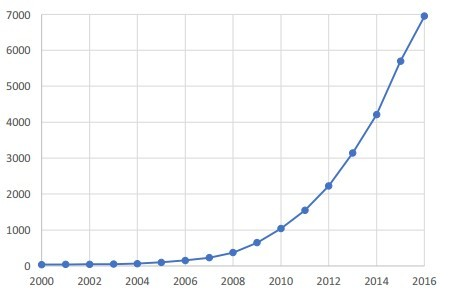
\includegraphics[width=8cm]{papersCountHistory.jpg}
    \caption{Cumulative count of papers about sentiment analysis}%
    \label{fig:papersCountHistory}%
\end{figure}



\section{Training datasets}
One of the main building blocks of any correctly and accurately functioning ML projects is a training phase. It can actually be seen as a base for the whole project. One can have the best fine-tuned optimized classifier, but if the training data he used do not fit the domain where the classifier is intended to be used, results of the classifier can be (surprisingly) bad. It's the same as house and its base. If the base is not done correctly, however cool architectural solution have other storeys used, house is still going to fall in the next big storm.

That's why choosing a sufficient and fitting dataset to train my classifiers was a very important task. The datasets I've considered were:
\begin{itemize}
  \item \textbf{Dataset140}\footnote{http://cs.stanford.edu/people/alecmgo/trainingandtestdata.zip} - it is currently the biggest dataset with tweets labeled by their sentiment. What is interesting and makes the dataset special is that opposed to other datasets being manually annotated by humans, this one was created by a program. It contains 1.6 million tweets with their polarity score (0 = negative, 2 = neutral, 4 = positive), tweet id, date of tweet publication, author of the tweet and the text of the tweet. More about how this dataset was created can be found in Go et al. paper \cite{go2009twitter}
  \item \textbf{Movie review data}\footnote{http://www.cs.cornell.edu/people/pabo/movie-review-data/} - Thousand positive and thousand negative labeled movie reviews. This dataset was introduced in Pang/Lee ACL 2004 \cite{pang2004sentimental}
  \item \textbf{Hu-Liu lexicon}\footnote{https://github.com/woodrad/Twitter-Sentiment-Mining/tree/master/Hu\%20and\%20Liu\%20Sentiment\%20Lexicon} - plain list of 6800 common English words labeled as positive and negative
  \item \textbf{Warriner et al lexicon}\footnote{http://crr.ugent.be/archives/1003} - This list of words was collected with Amazon Mechanical Turk. Three components of emotions are distinguished: valence (the pleasantness of a stimulus), arousal (the intensity of emotion provoked by a stimulus), and dominance (the degree of control exerted by a stimulus) \cite{warriner2013norms}. Warriner and Kuperman extended ANEW norms collected by Bradley and Lang from 1034 words to 13,915 words (lemmas).
  \item \textbf{Stack overflow dataset}\footnote{https://sentiment-se.github.io/replication.zip} - Later into the thesis I've decided to test dataset of 1500 manually labeled Stack overflow sentences created by Bin Lin et al. in their late paper on negative results in SA called "How far can we go".
    \item \textbf{My own cryptocurrency tweets dataset} - As already said before, performance of the classifier depends on how close the training data are to the real use-case data. That's why I considered and even started to create my own dataset targeting specifically only cryptocurrency tweets, which I've intended to analyze as well.
\end{itemize}

Big surprise here was the lack of any bigger Reddit dataset.

\section{Language processing tools}
From the very beginning, I knew I wanted to use Python. I had some slight background knowledge in ML from online courses and most of them were done in Python. Therefore while searching and deciding which library should I use, I've always given a slight edge to the Python options. I've considered (and tested) these:
\begin{itemize}
\item \textbf{NLTK} - probably the best-known Python module for NLP. It provides easy-to-use interfaces for more than 50 corpora and lexical resources. It also offeres a rich palette of processing libraries for classification, tokenization, stemming, tagging, parsing, and semantic reasoning.
\item \textbf{Textblob: Simplified Text Processing} - as a name says, Textblob provides easy processing and is actually built on top of NLTK. It provides a simple API for diving into common natural language processing tasks such as part-of-speech tagging, noun phrase extraction, sentiment analysis (Naive Bayes, Decision Tree), classification, translation and more.
\item \textbf{Scikit-learn} - Python module for general ML, data mining and data analysis. It is built on NumPy, SciPy and matplotlib modules.
\end{itemize}

Also, sentiment analysis is just one part of the task. To evaluate the data and find pattern, basic data science algorithms will be needed. With data science, R is very often listed as a default choice. Therefore were the results of google trends query shown in Figure  pretty surprising. This definitely helped my decision with sticking to Python.

\begin{figure}[H]%
    \centering
	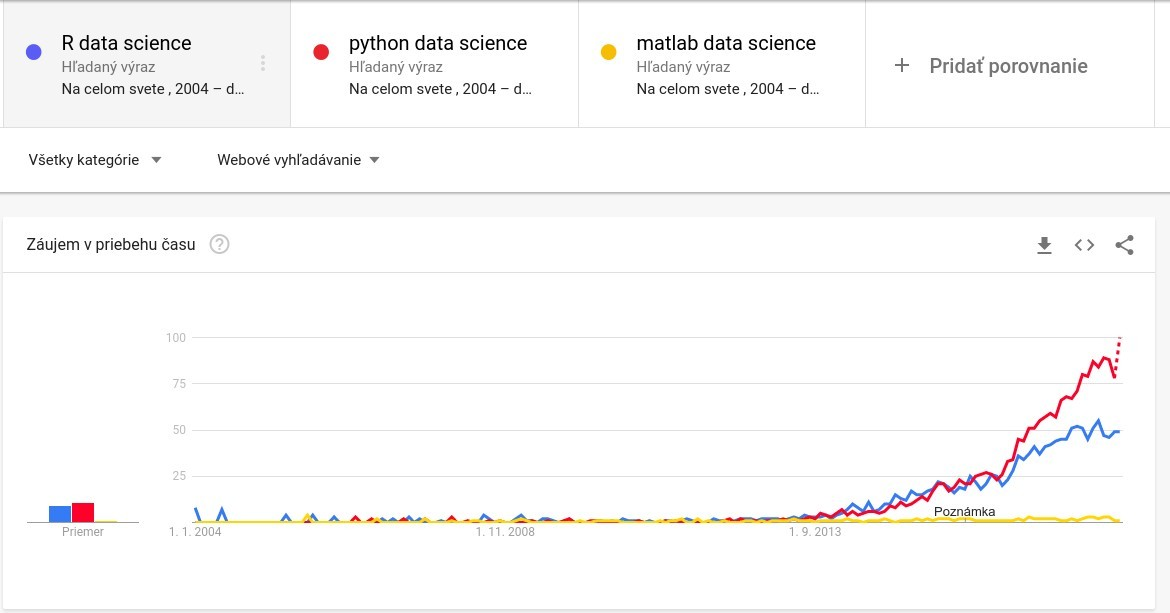
\includegraphics[width=10cm]{PythonMatlabR.jpg}
    \caption{Google trend of searches regarding data science with various programming languages}%
    \label{fig:PythonMatlabR}%
\end{figure}


\section{Performance metrics}
\paragraph{Terminology} Before diving into talk about the metrics, there are 4 crucial terms which need to be explained:
\begin{itemize}
\item \textbf{Tue Positives (TP)} - instances correctly labeled as positive
\item \textbf{True Negatives (TN)}- instances correctly labeled as negative
\item \textbf{False Positives (FP)} - instances incorrectly labeled as positive
\item \textbf{False Negatives (FN)}- instances incorrectly labeled as negative
\end{itemize}


The metrics that you choose to evaluate your machine learning algorithms are very important and not all are suitable for every situation. Choice of metrics influences how the performance of machine learning algorithms is measured and choosing a wrong evaluation metric for particular use could potentially lead towards eliminating the best performing algorithm in favour of the worse one.
Here are some of the most often used metrics used to evaluate classification algorithms. It's also useful to choose the metric before doing the analysis, so you won't get distracted by already having the results in case of doing the decision later.

\begin{itemize}
\item \textbf{Classification accuracy} - this is the most intuitive and common evaluation metric for classification problems but it is also the most misused one. It is really only suitable when there are an equal number of observations in each class (which is rarely the case) and that all predictions and prediction errors are equally important, which is often not the case. In case of imbalanced dataset with 9\% of instances in one class and only 10\% in the other, predicting every instance as a majority class without even considering its features would lead to high accuracy of 90\%. This is called \textbf{accuracy paradox.}
\[ Accuracy = \frac{TP + TN}{TP + TN + FP + FN}\]
\item \textbf{Confusion matrix} - clean and unambiguous way to present the prediction results of a classifier. If the classification is binary (there are only 2 classes), this matrix has 2 rows and 2 columns - therefore altogether 4 cells which are filled with true/false positives/negatives count. Such scenario is demonstrated in table \ref{table:Confusion_matrix_general}. Although the confusion matrix shows all of the information about the classifier's performance, more meaningful measures can be extracted from it to illustrate certain performance criteria.\cite{bradley1997use}. 
\begin{table}[H]
{
\centering
\begin{tabular}{ |p{4cm}|p{4cm}|p{4cm}|  }
 \hline
 \multicolumn{3}{|c|}{Confusion matrix} \\
 \hline
  & Predicted positive & Predicted negative\\
 \hline
 Real positive   & TP    &FN\\ \hline
 Real negative &   FP  & TN\\ \hline
\end{tabular}
}
\caption{Confusion matrix}
\label{table:Confusion_matrix_general}
\end{table}

\item \textbf{Precision} - Precision can be seen as a representation of a classifiers exactness. A low precision can also indicate a large number of False Positives. If the precision is high, it says that there's a high probability of positive label being True Positive. It cannot be tricked but it also hides a lot.
\[ Precision = \frac{TP}{TP + FP}\]
\item \textbf{Recall} - also called \textit{sensitivity} or the \textit{True Positive Rate}, it is a number of True Positives divided by the number of True Positives and the number of False Negatives. In other words, it is a ratio of how many of all positive instances have been identified. Recall can be tricked (labeling all as majority class) but if used next to precision, it gives extra information
\[ Recall = \frac{TP}{TP + FN}\]
\item \textbf{F measure} - as already mentioned, precision hides some facts and recall can be tricked. To give the full story, they need to be used together. That's what F measure is for.
\[ F = 2 * \frac{precision * recall}{precision + recall}\]
\end{itemize}Nice example to demonstrate difference between precision and recall is the concept of Indian Jurisprudence, where "100 culprits may let go free but no innocent should be punished". If we let go so many culprits in order to ensure no innocent is punished, recall will be pretty low, but precision very high.


\section{Results}

\subsection{Cross-correlation between releases and sentiment change}
When working with time series, we often want to determine whether one series causes changes in another. To find this relationship, measuring a cross-correlation and finding a lag is one way how to do it. Lag represents when change in one data series transfers to the other several periods later. 

To ensure a cross-correlation calculation makes sense, first I have to determine, whether are the data stationary. A stationary time series is one whose properties do not depend on the time at which the series is observed\cite{hyndman5forecast}. More precisely, if y\textsubscript{t} is a stationary time series, then for all \textit{s}, the distribution of \textit{(y\textsubscript{t},…,y\textsubscript{t+s})} does not depend on \textit{t}.

To determine whether my data are stationary, I've used the Dickey-Fuller test method of tseries package in R. Results can be seen in the table \ref{table:stationarity_table_sentiment} and \ref{table:stationarity_table_release_count} 

\begin{table}[H]
\centering
\begin{tabular}{ |p{3cm}||p{3cm}|p{3cm}|  }
 \hline
 \multicolumn{3}{|c|}{Stationarity test of web frameworks sentiment data} \\
 \hline
 Framework & Dickey-Fuller & p-value\\
 \hline
 NodeJS   & -2.6775    &0.2964\\ \hline
 AngularJS &   -3.883  & 0.0199\\ \hline
 EmberJS & -4.0783 & 0.0199\\ \hline
 VueJS    &-3.438 & 0.0646\\ \hline
 CakePHP&   -3.480  & 0.04847\\ \hline
 Laravel& -2.57  & 0.3431\\ \hline
 Symfony& -4.3979  & 0.01\\ \hline
\end{tabular}
\caption{Stationarity test of sentiment}
\label{table:stationarity_table_sentiment}
\end{table}

\begin{table}[H]
\centering
\begin{tabular}{ |p{3cm}||p{3cm}|p{3cm}|  }
 \hline
 \multicolumn{3}{|c|}{Stationarity test of web frameworks release count} \\
 \hline
 Framework & Dickey-Fuller & p-value\\
 \hline
 NodeJS   & -2.896    &0.205\\ \hline
 AngularJS &   -2.547  & 0.353\\ \hline
 EmberJS & -3.297 & 0.0802\\ \hline
 VueJS    &-2.158 & 0.511\\ \hline
 CakePHP&   -3.224  & 0.08915\\ \hline
 Laravel& -2.368  & 0.425\\ \hline
 Symfony& -2.218  & 0.488\\ \hline
\end{tabular}
\caption{Stationarity test of release counts}
\label{table:stationarity_table_release_count}
\end{table}

As we can see, p-values are always higher than 0.05 what indicates non-stationarity of the data, therefore I can't calculate the cross-correlation on them in this state. To transform non-stationary data into stationary, 2 approaches can be used. These are differencing and transforming.  I've taken data series and differenced the values in listing \ref{lst:differencing}. I've executed both, seasonal differencing and stationary differencing although seasonal probably was not needed because the data should not be dependant on the season.

\begin{lstlisting}[caption={Used differencing method in R},label={lst:differencing},language=R]
Differencing <- function(x,y)
{
 framework_x_seasdiff <- diff(x,differences=1)  # seasonal differencing
 framework_x_Stationary <- diff(framework_x_seasdiff, differences= 1)
 framework_y_seasdiff <- diff(y, differences=1)
 framework_y_Stationary <- diff(framework_y_seasdiff, differences= 1)
 return(list(framework_x_Stationary,framework_y_Stationary))
}
\end{lstlisting}
New differenced values do appear to be stationary in mean and variance, as the level and the variance of the series stays roughly constant over time. Sentiment for NodeJS before and after differencing can be seen in Figure \ref{fig:NodeJS_Sentiment_before_after}

\begin{figure}[H]%
    \centering
    \subfloat[Before differencing]{{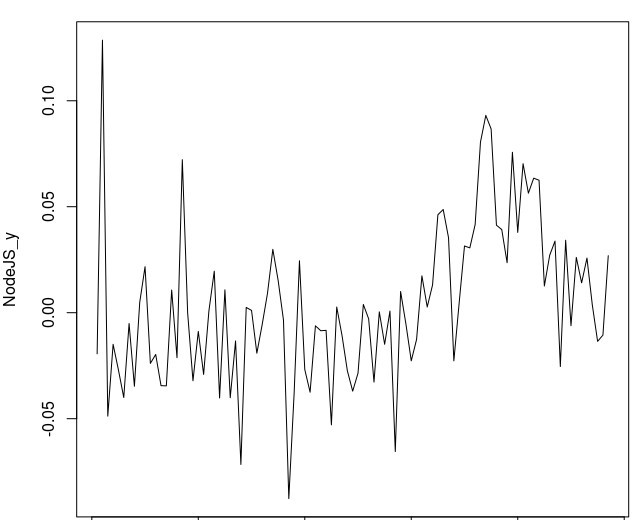
\includegraphics[width=6cm]{NodeJS_before.jpg} }}%
    \qquad
    \subfloat[After differencing]{{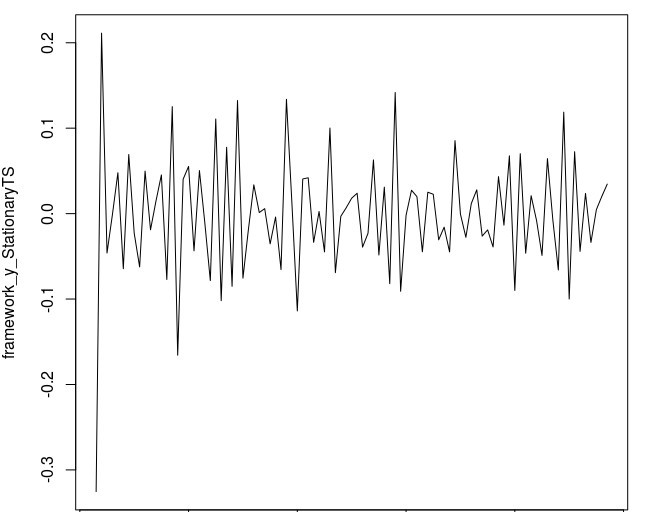
\includegraphics[width=6cm]{NodeJS_after.jpg} }}%
    \caption{NodeJS monthly sentiment values}%
    \label{fig:NodeJS_Sentiment_before_after}%
\end{figure}

Same procedure needed to be done with the "number of releases per month" data and afterwards. Then, cross-correlation could be executed. For this task I've used ccf method in R which implements Pearson's correlation calculation method. Results for all 7 OSS projects can be seen in Figure \ref{fig:highestCorrelationsPlotReleases}

\begin{figure}[H]%
    \centering
	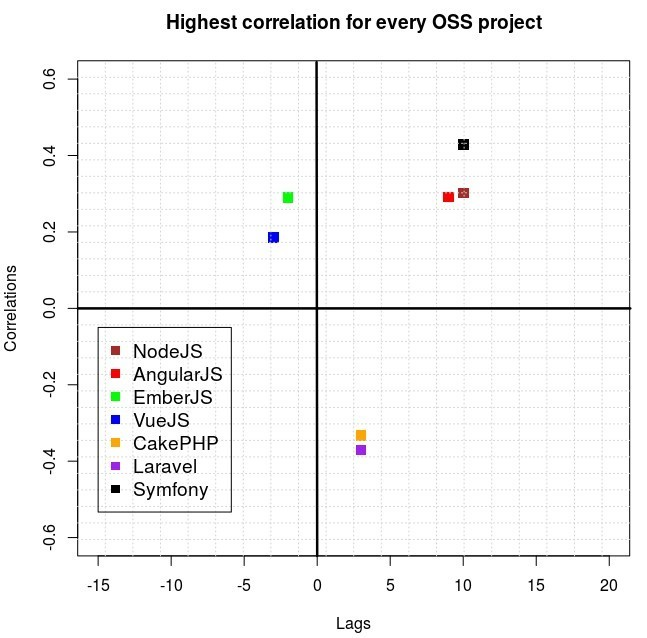
\includegraphics[width=8cm]{highestCorrelationsPlotReleases.jpg}
    \caption{Highest correlations for every OSS project}%
    \label{fig:highestCorrelationsPlotReleases}%
\end{figure}

\paragraph{Results interpretation:}

As we can there is no general pattern. Maximal project correlations happen to occupy 3 of 4 possible quadrants. Each quadrant represents a different relationship between number of releases and sentiment change.

\begin{itemize}
  \item \textbf{I. Quadrant}(Positive correlation + positive lag) - Increase of release count increases a sentiment
  \item \textbf{II. Quadrant}(Positive correlation + negative lag) - Increase of sentiment increases a release count
  \item \textbf{III. Quadrant}(Negative correlation + positive lag) - Increase of release count decreases a sentiment
  \item \textbf{IV. Quadrant}(Negative correlation + Negative lag) - Increase of sentiment decreases a release count
\end{itemize}

Also, in Figure \ref{fig:highestCorrelationsPlotReleases_nonStat} are the results without making the data series stationary. It's obvious that making the data stationary has a big impact on the results.

\begin{figure}[H]%
    \centering
	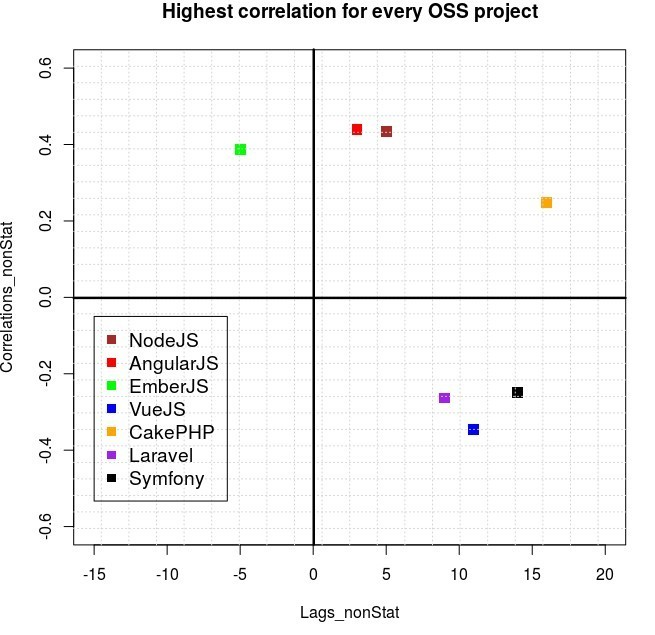
\includegraphics[width=8cm]{highestCorrelationsPlotReleases_nonStat.jpg}
    \caption{Highest correlations for every OSS project (non-stationary)}%
    \label{fig:highestCorrelationsPlotReleases_nonStat}%
\end{figure}

\subsection{Commits count within releases} \label{ssec:crossCorrelationCommits}
Initially, I thought that to modify project to take into account a size of the release (amount of commits) will be pretty straightforward task. It actually was straightforward, but as always I've encountered several unexpected problems on the way. \\
I intended to extend my previously used method from Section \ref{ssec:gitReleaseDatesMining} which uses Git API tags endpoint to get the release dates. Unfortunately I wasn't able to find number of commits in the returned objects. JSON object returned from API has following structure:
\begin{lstlisting}
  {
    "url": X,
    "assets_url": X,
    "upload_url": X,
    "html_url": X,
    "id": X,
    "tag_name": X,
    "target_commitish":X,
    "name": X,
    "draft": X,
    "author":{},
    "prerelease": X,
    "created_at": X,
    "published_at": X,
    "assets":[],
    "tarball_url": X,
    "zipball_url":X, 
    }
\end{lstlisting}
I have done some extra searching but did not want to spend extra time so I decided to go the way I knew will work. Instead of using API to get the commit counts, I crawled GitHub UI page of each release and extracted information directly from page source code. Each release details page provides information how many commits behind the current HEAD the commit is. The difference in this number between two following releases represents count of new commits for a release. Results of simple tabular substraction with spreadsheet formula needed to be manually corrected because projects often release several branches parallel and therefore substraction from the previous release was not always the correct one.\\
\\
Eventually, I got correct number of commits for every release and could execute the same cross-correlation analysis described in the previous chapter, but this time instead of releases count, I have explored relationship between sentiment and commits count. One possible flaw in the commit count data are the pre-releases. I treated them as normal releases because they do offer new features but those very same commits are then counted in the official releases later on.\\
\\
After getting the data ready I performed a stationarity test for commit counts. Sentiment values are the same as before with count of releases. Table \ref{table:stationarity_table_commits} shows the results.

\begin{table}[H]
\centering
\begin{tabular}{ |p{3cm}||p{3cm}|p{3cm}|  }
 \hline
 \multicolumn{3}{|c|}{Stationarity test of web frameworks commit counts} \\
 \hline
 Framework & Dickey-Fuller & p-value\\
 \hline
 NodeJS   & -7.0239    &0.01\\ \hline
 AngularJS &   -2.547  & 0.3531\\ \hline
 EmberJS & -3.2764 & 0.0831\\ \hline
 VueJS    &-2.9748 & 0.1886\\ \hline
 CakePHP&   -3.655  & 0.03283\\ \hline
 Laravel& -2.919  & 0.2084\\ \hline
 Symfony& -4.8461  & 0.01\\ \hline
\end{tabular}
\caption{Stationarity test of commit counts}
\label{table:stationarity_table_commits}
\end{table}

I see that there are again several data series (AngularJS, EmberJS, VueJS, Laravel + NodeJS because of unstationarity of sentiment data) which are not stationary so exactly as before with release counts, I had to transform the data. After that, Pearson's cross correlation was calculated. Results for all 7 OSS projects can be seen in Figure \ref{fig:highestCorrelationsPlot}

\begin{figure}[H]%
    \centering
	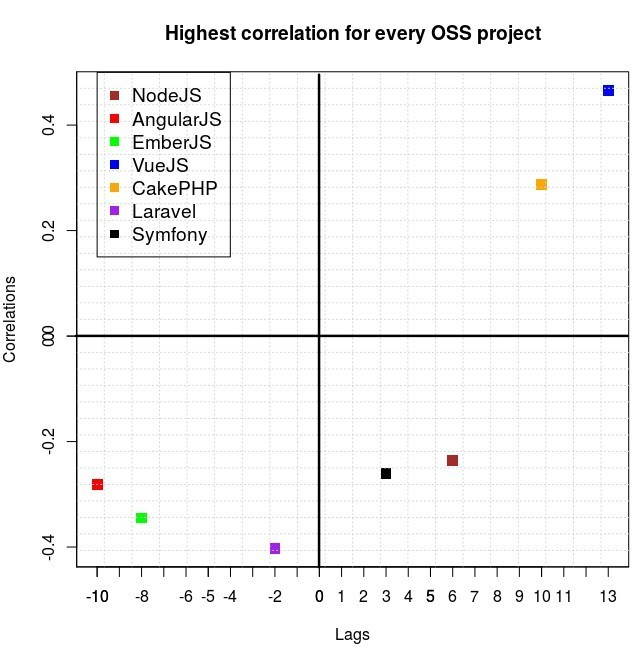
\includegraphics[width=8cm]{highestCorrelationsPlot.jpg}
    \caption{Highest correlations for every OSS project}%
    \label{fig:highestCorrelationsPlot}%
\end{figure}

If I would skip the step of making the data stationary, results would again look completely different \ref{fig:highestCorrelationsPlot_nonStat}.

\begin{figure}[H]%
    \centering
	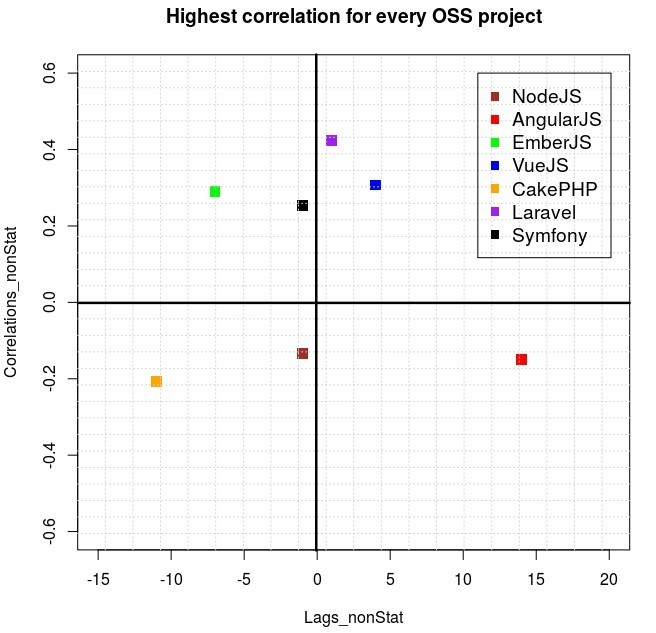
\includegraphics[width=8cm]{highestCorrelationsPlot_nonStat.jpg}
    \caption{Highest correlations for every OSS project (non-stationary)}%
    \label{fig:highestCorrelationsPlot_nonStat}%
\end{figure} 


\chapter{Pairing bugs}
\label{chp:pairingBugs}
My goal of pairing bugs with social media might be somewhat similar to nowadays very active field of bug report duplicate discovery but has also a lot common with topic modeling and general text similarity algorithms.

To link any two texts based on their content, there's an obvious need for understanding what the text features are. 
To do this, there are several ways how to calculate text (string) similarity value or one can even execute so called "Topic modeling" algorithm and try to connect documents based on their matching topics.

Topic modeling is a method used to organize and summarize large textual information. It's used to discover hidden topical patterns and annotate documents according to these topics. It can also be described as a method of finding group of words (i.e topic) from in a text that best represents the information in the collection.

The obstacle of using a topic modeling for my case is that neither SO nor Reddit questions are not long enough. This could potentially be avoided by concatenating the whole discussions into one long text but these are still too topic-specific to get reasonable output. In this case, topic modeling output is not granular enough to differentiate among similar texts which are all from the very same domain. 

Because the output provided by topic modeling wasn't enough to pair particular items, I searched for, found and considered several alternative approaches.

\section{Aproaches}
There are many ways and approaches how to find out whether 2 texts share some common topic. Most of them are to some extent very similar as the general rule is to extract textual features and compare them using statistical approaches. Common way to do this is to transform documents into vectors and then compute cosine similarity between them. These text transformations are implemented in several Python packages.\\
\\
I have tried following:
\begin{enumerate}
\item String similarity using NLTK
\item String similarity using Scikit-learn
\end{enumerate}

\paragraph{NLTK:}First step in calculating similarity was to tokenize the text. NLTK offers several types of tokenizers with various outputs. Text tokenization can operate on various levels and the structure of input has to be considered. As I am comparing the whole documents and do not want to consider sentences as standalone objects, I have chosen to use \textit{nltk.tokenize.wordtokenize} method instead of e.g. \textit{nltk.tokenize.senttokenize}.\\
Next step after the document is tokenized is to stem the words. Stemmers remove morphological affixes from words, leaving only the word stem. Once again as with tokenizers, there are several stemmers implemented within NLTK. After doing a short research I have come to conclusion that as far as I use the same stemmer for both, Git issues and SO/Reddit entries, it should not play any major role in results.\\
Next step is getting rid of stop words. These usually refer to the most common words in a language, but there is no single universal list of stop words used by all natural language processing tools. The set of stop words defined for my NLTK version had a size of 153.\\
Listing \ref{lst:nltkTextSimilarity} illustrates the implementation of the described similarity calculation procedure.

\begin{lstlisting}[caption={Text similarity implementation with NLTK},label={lst:nltkTextSimilarity},language=Python]
		tokens = word_tokenize(text)
		words = [w.lower() for w in tokens]

		porter = nltk.PorterStemmer()
		stemmed_tokens = [porter.stem(t) for t in words]

		# removing stop words
		stop_words = set(stopwords.words('english'))
		filtered_tokens = [w for w in stemmed_tokens if not w in stop_words]

		# count words
		count = nltk.defaultdict(int)
		for word in filtered_tokens:
			count[word] += 1
		return count;
\end{lstlisting}

After the previous 3 steps are executed on both documents, 2 vectors from all words from both documents are created. Each documents then sets the counts of words it contains and a cosine similarity of these two "count vectors" is calculated. This similarity calculation is a basic similarity calculation and could definitely be optimized. For example, it does not analyse and consider role and position of word in a sentence (POS tagger would be required here). 

\paragraph{Scikit-learn and TF-IDF:}There are several ways to assess the importance of each feature by attaching a certain weight in the text. The most
popular ones are: feature frequency (FF), Term Frequency Inverse Document Frequency (TF-IDF), and feature presence
(FP) \cite{haddi2013role}. My next similarity checker I have implemented was using Scikit-learn module and TF-IDF vectorizer. While BoG only takes into consideration the frequency of words in a document TF-IDF reflects how important a word is for the particular document. For a word to have high TF-IDF in a document, it must appear a lot of times in said document and must be absent in the other documents. It must be a signature word of the document.\\
\\
Term frequency represents how often is the word present in the said document. Simplest approach is the raw count.
\[ tf_{count}(t,d) = f(t,d) \]
Other options include term frequency adjusted for document length, logarithmically scaled frequency or augmented frequency to handle bias towards longer documents.\\
Inverse document frequency is a counterweight factor which diminished importance of terms that appear in the set very often in the document set and therefore increases the weight of terms that occur rarely.
\[ idf(t) = log \frac{N}{df(t)} \]
The final weighing scheme combines term frequency and inverse document frequency.
\[ tfidf(t,d) = tf(td) x idf(t)		\]
Listing \ref{lst:scikitkTextSimilarity} shows my very simple implementation of TF-IDF similarity checker using Scikit-learn module.

\begin{lstlisting}[caption={Text similarity implementation with Scikit using Tf-Idf model},label={lst:scikitkTextSimilarity},language=Python]
		def getSimilarity(self,text1, text2):
			tfidf = self.vect.fit-transform([text1, text2])
			return (tfidf * tfidf.T).A
\end{lstlisting}

\paragraph{Stack Overflow questions preprocessing:}  Online texts contain usually lots of noise and uninformative parts such as HTML tags, scripts and advertisements \cite{haddi2013role}. Before running implemented similarity algorithms, I have decided to preprocess the stack questions and get rid of code snippets within \textit{\textless pre\textgreater\textless code\textgreater} tags and hypertext links. Especially snippets could potentially effect (increase) the similarity score if kept in the text.

	

\section{Available data}
\paragraph{Git issue reports:}
Using the approach described in the section \ref{ssec:issuesMining}, I've downloaded 96,651 issue reports from Git while 25,978 of those labeled as bug or similar. Because this part of the thesis was more just a PoC than the part with sentiment analysis, I've decided not to work with all the data and rather just picked several projects of interest. The bug counts among this projects is displayed in the table \ref{table:projectIssuesDistribution}.


\begin{table}[H]
\centering
\begin{tabular}{ |p{3cm}||p{3cm}|}
 \hline
\textbf{ Framework }& \textbf{Bug count}\\
 \hline
 NodeJS   & 1615\\ \hline
 AngularJS &   2225 \\ \hline
 EmberJS & 1284\\ \hline
 VueJS & 353\\ \hline
 Aurelia & 73\\ \hline
 Bower & 155\\ \hline
\end{tabular}
\caption{Bug count per project}
\label{table:projectIssuesDistribution}
\end{table}

\paragraph{Stack overflow questions:}
SO mining has been described in section \ref{ssec:GettingData} and I've downloaded 5,847 questions. There are thousand questions for AngularJS, NodeJS, Bower, Ruby on Rails and VueJS each and EmberJS has only 847 questions. Downside is, that despite having a lot of questions, it doesn't necessarily mean that each and every one of them talks about some known bug. Actually, opposite is true as out of all those questions only very tiny percentage does (AngularJS - 1, NodeJS - 2, EmberJS - 2, VueJS - 0).

\paragraph{Reddit dialogues:}Reddit subreddits mining has been described in the same subsection as SO mining. Results of this process are shown in the table \ref{table:redditDiscussionsDistribution}.


\begin{table}[H]
\centering
\begin{tabular}{ |p{3cm}||p{3cm}|}
 \hline
\textbf{ Framework }& \textbf{Submissions count}\\
 \hline
 NodeJS   &  108\\ \hline
 AngularJS &   43 \\ \hline
 VueJS & 20\\ \hline
 EmberJS & 13\\ \hline
\end{tabular}
\caption{Reddit submissions counts}
\label{table:redditDiscussionsDistribution}
\end{table}


\section{Similarity results}
Linking items and in general finding similarity among these already area-specific texts proved to be a problematic task. To test my algorithm I decided to compare 89 SO questions with its matching Git issue and 4x one random git issue of the project. Results are plotted in Figure \ref{fig:MatchesVsRandom}.\\

\begin{figure}[H]%
    \centering
	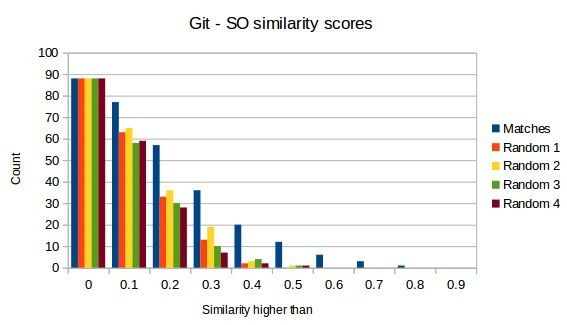
\includegraphics[width=15cm]{MatchesVsRandom.jpg}
    \caption{Similarity distribution of 89 matches and four data series of 89 random pairs}%
    \label{fig:MatchesVsRandom}%
\end{figure}
Results very clearly show that there is a particular similarity score, which is very hard to pass for two unrelated items. This score is obviously not constant and it depends on implementation of the similarity calculation. For my NLTK BoW algorithm used in Figure \ref{fig:MatchesVsRandom}, the threshold is 0.4 or 0.5. Choosing the value of threshold would also depend on the  desired characteristics of a classifier and the prioritized metric. For example if a precision would be more important than recall, the ideal threshold would be 0.7 as it is the value which has never been passed by any of 356 non-matching pairs. The detailed table with the values for a Figure \ref{fig:MatchesVsRandom} can be seen in appendix.\\
\\
I have executed the same steps using the TF-IDF approach and although the values are different (as expected), they follow the same pattern. Figure \ref{fig:MatchesVsRandom_TfIdf} demonstrates these results and detailed values can again be found in appendix.

\begin{figure}[H]%
    \centering
	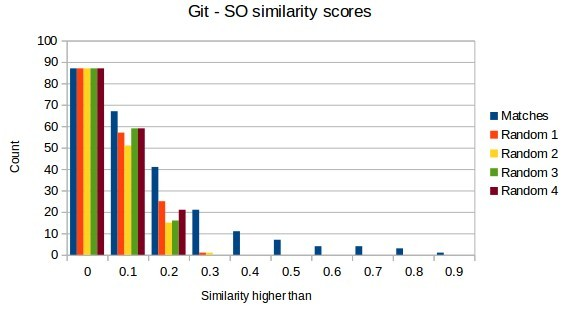
\includegraphics[width=15cm]{MatchesVsRandom_TfIdf.jpg}
    \caption{Similarity distribution of 89 matches and four data series of 89 random pairs}%
    \label{fig:MatchesVsRandom_TfIdf}%
\end{figure}

Despite clearly seeing possible threshold values, an algorithm which would label all the pairs above this threshold as matches would achieve very bad recall around 30\%. On the other side, precision would be 100\%. The potential problem is that the real-world ratio between matching and non-matching pairs rises exponentially with every new item on any side (Git issue, SO question). Testing the algorithm on bigger amount of data in the future could answer the question whether the threshold around 0.3 really proves as a unbreakable resistance for unrelated Git-SO pairs.\\
\\
Although I was not successful to such extent that the output are Git-StackOverflow or Git-Reddit True Positive pairs, I have pointed out some interesting results and data relationships.

\label{ssec:similarityResultsSO}
\subsection{Stack Overflow}
The average similarity (using NLTK approach) between SO questions talking about particular issue and that particular issue description is 0.316 without body preprocessing and 0.292 with body preprocessing. The distribution of similarities in buckets by increased by 0.05 can be seen in histogram in Figure \ref{fig:GitStackMatchesHistogram}

\begin{figure}[H]%
    \centering
	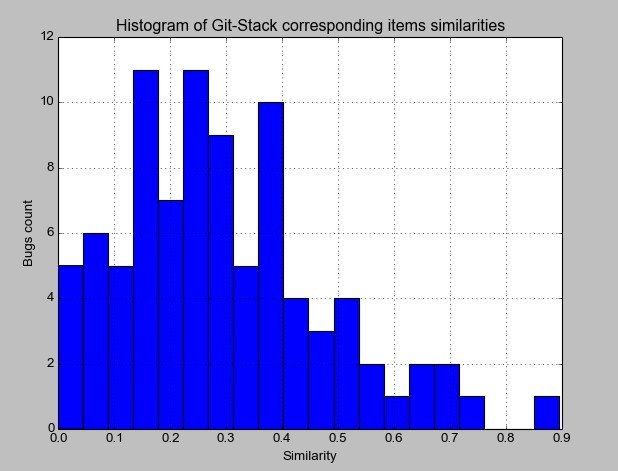
\includegraphics[width=8cm]{gitStackMatchesHistogram.jpg}
    \caption{Histogram of similarities distribution among git issues and their matching SO questions}%
    \label{fig:GitStackMatchesHistogram}%
\end{figure}

For random SO questions, amount of comparisons to Git issues needed to be limited. If every SO question would be compared to every Git issue, time of computation would exceed timeframe of this thesis. Every SO question was therefore compared to 20 random Git issues and resulting average similarity scores are in following figures.

\begin{figure}[H]%
    \centering
	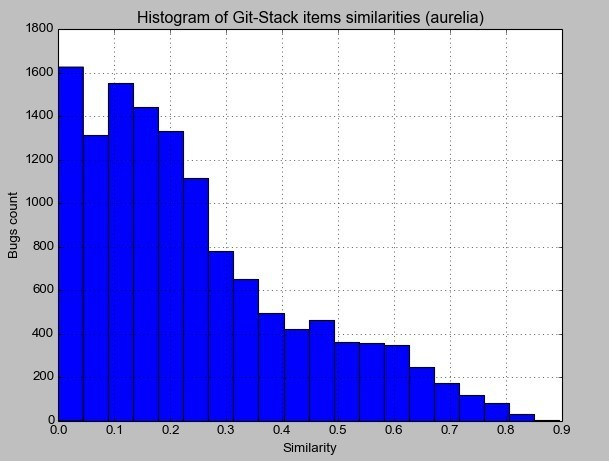
\includegraphics[width=8cm]{AureliaStackWithRandom20Bugs.jpg}
    \caption{Histogram of Aurelia SO questions and random git issues. Average similarity was 0.244}%
    \label{fig:AureliaStackWithRandom3Bugs}%
\end{figure}

\begin{figure}[H]%
    \centering
    \subfloat[EmberJS average similarity - 0.247]{{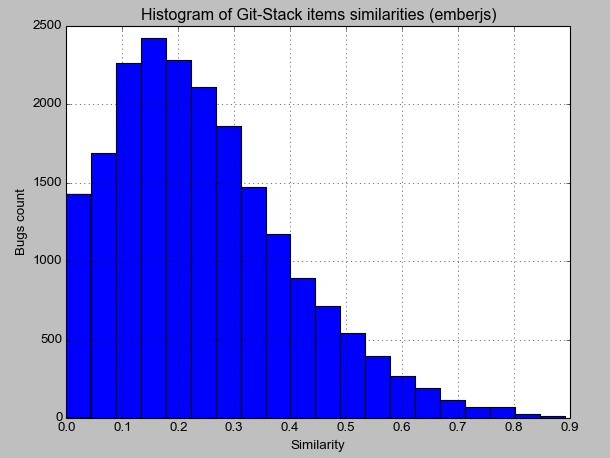
\includegraphics[width=5.5cm]{EmberStackWithRandom20Bugs.jpg} }}%
    \qquad
    \subfloat[Bower average similarity - 0.217]{{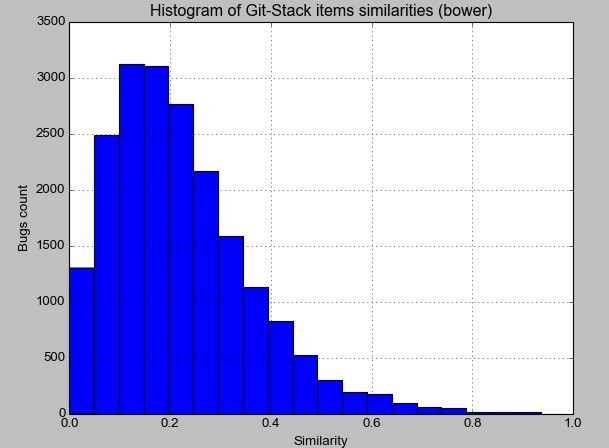
\includegraphics[width=5.5cm]{BowerStackWithRandom20Bugs.jpg} }}%
    \caption{EmberJS and Bower similarity histogram}%
    \label{fig:BowerEmberWithRandom3Bugs}%
\end{figure}

\begin{figure}[H]%
    \centering
    \subfloat[VueJS average similarity - 0.255]{{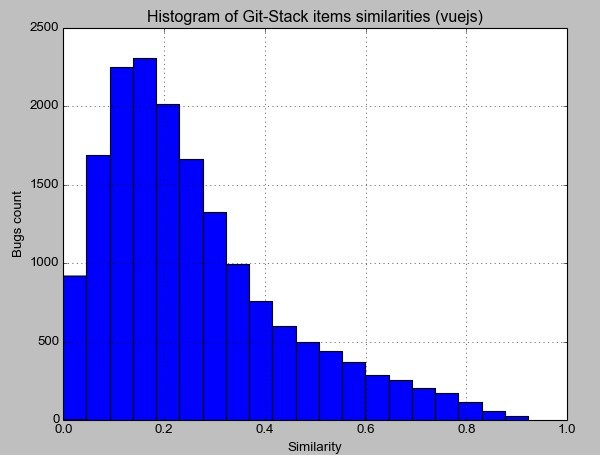
\includegraphics[width=5.5cm]{VueJSStackWithRandom20Bugs.jpg} }}%
    \qquad
    \subfloat[AngularJS average similarity - 0.258]{{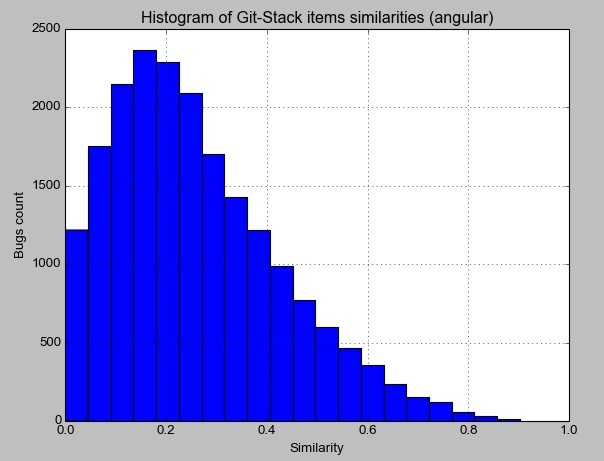
\includegraphics[width=5.5cm]{AngularStackWithRandom20Bugs.jpg} }}%
    \caption{VueJS and AngularJS similarity histogram}%
    \label{fig:VueAngularWithRandom3Bugs}%
\end{figure}


Table \ref{table:StackOverflowNLTKsimilarity} illustrates results of comparing Git bugs descriptions with SO questions talking about the same project issues and general issues. From values displayed, it is apparent that the difference between matches and random pairs is not very big. This is probably because all the texts about a particular project are already very specific and similar in their nature anyway.

\begin{table}[H]
\centering
\begin{tabular}{ |p{3cm}||p{4.5cm}|p{5.5cm}|}
 \hline
\textbf{ Framework }& \textbf{Own issues similarity}& \textbf{20 random issues similarity}\\
 \hline
 NodeJS   & 0.265 & 0.243\\ \hline
 AngularJS & 0.241 & 0.260\\ \hline
 EmberJS & 0.282 & 0.246\\ \hline 
 VueJS &   0.261 & 0.258\\ \hline
\end{tabular}
\caption{NLTK similarity values for SO questions}
\label{table:StackOverflowNLTKsimilarity}
\end{table}

\subsection{Reddit}Here I have calculated the similarity between the bug description and either particular comment in the Reddit discussion which mentioned the bug or the whole discussion itself. Using NLTK BoW approach, average similarity score for all considered projects (NodeJS, AngularJS, VueJS and EmberJS) was 0.481 for the whole discussion and 0.368 for the comment itself. Scikit If-Idf values were 0.263 and 0.207 respectively. Detailed scores for each project can be found in Table \ref{table:RedditNLTKsimilarity} for NLTK implementation and Table \ref{table:RedditSCIKITsimilarity} for Sci-kit. Subreddit for EmberJS did not reference any of its own bugs.

\begin{table}[H]
\centering
\begin{tabular}{ |p{3cm}||p{3cm}|p{4cm}|}
 \hline
\textbf{ Framework }& \textbf{Bug comment}& \textbf{Whole discussion}\\
 \hline
 NodeJS   & 0.447 & 0.507\\ \hline 
 AngularJS & 0.306 & 0.57 \\ \hline 
 VueJS &   0.359 & 0.380\\ \hline
\end{tabular}
\caption{Reddit NLTK similarity values}
\label{table:RedditNLTKsimilarity}
\end{table}

\begin{table}[H]
\centering
\begin{tabular}{ |p{3cm}||p{3cm}|p{4cm}|}
 \hline
\textbf{ Framework }& \textbf{Bug comment}& \textbf{Whole discussion}\\
 \hline
 NodeJS   & 0.255 & 0.328\\ \hline 
 AngularJS & 0.168 & 0.278 \\ \hline 
 VueJS &  0.209  & 0.208\\ \hline
\end{tabular}
\caption{Reddit Scikit similarity values}
\label{table:RedditSCIKITsimilarity}
\end{table}

Both similarity calculations indicate that the semantic meaning of the bug is better expressed in the whole discussion rather than just the particular comment which referenced the bug. This made me question if it could be generalized that longer the text is, more similar it is to actual bug description. I have plotted a relationship between similarity score and length for Reddit in Figure \ref{fig:SimilarityLengthRelationshipComment} and the same for Stack Overflow discussion can be seen in Figure \ref{fig:GitStackSimilarityWeightedScatter}.

\begin{figure}[H]%
    \centering
    \subfloat[Discussion lengths]{{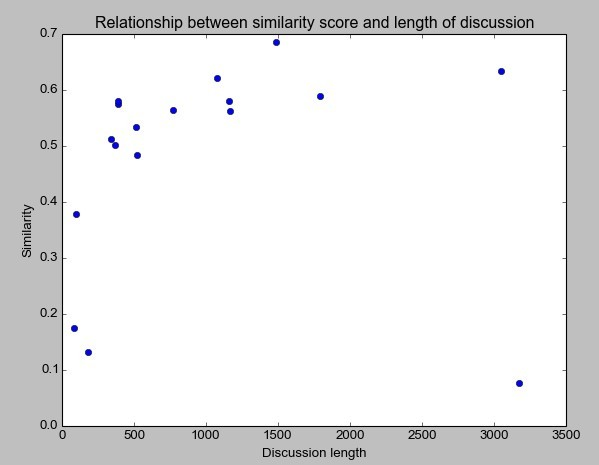
\includegraphics[width=5.5cm]{SimilarityLengthRelationshipDiscussion.jpg} }}%
    \qquad
    \subfloat[Comment lengths]{{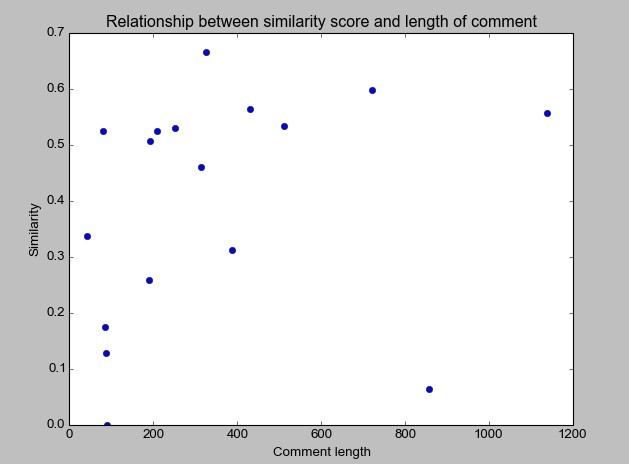
\includegraphics[width=5.5cm]{SimilarityLengthRelationshipComment.jpg} }}%
    \caption{Text lengths and similarity scores with matching issues}%
    \label{fig:SimilarityLengthRelationshipComment}%
\end{figure}

\begin{figure}[H]%
    \centering
	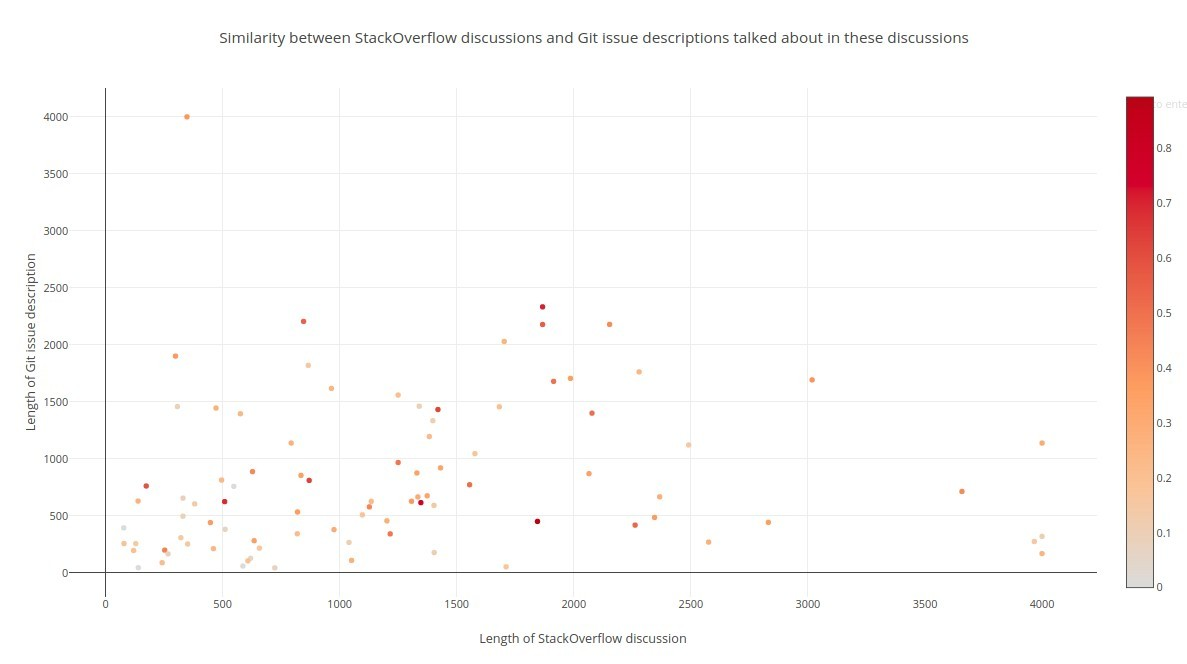
\includegraphics[width=10cm]{GitStackSimilarityWeightedScatter.jpg}
    \caption{Git and SO discussion lengths and similarity scores with the issue}%
    \label{fig:GitStackSimilarityWeightedScatter}%
\end{figure}


\section{Buckets}
ReBucket measures the similarities of call stacks in crash reports and then assigns the reports to appropriate buckets based on the similarity values.\cite{dang2012rebucket}


\section{Using GIT labels}
One more considered approach how to recognize an issue's topic was using the GIT labels. Labels on GitHub help you organize and prioritize your work. You can apply labels to issues and pull requests to signify priority, category, or any other information you find useful. There are two types of labels - default and custom. GitHub provides default ones in every new repository. All default labels can be seen in table \ref{fig:defaultLabels} and can be used to create a standard workflow in a repository:

\begin{figure}[H]%
    \centering
	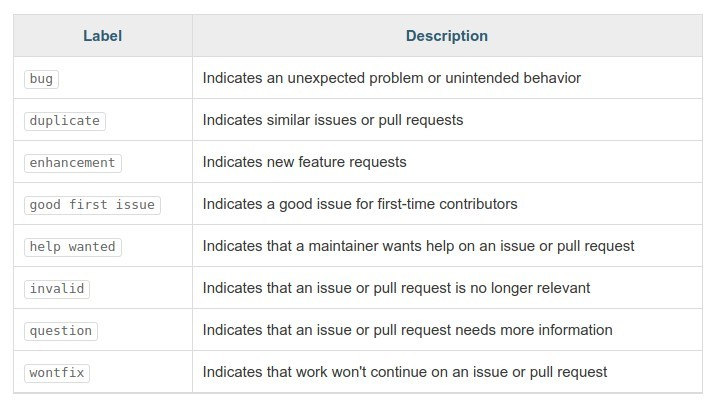
\includegraphics[width=8cm]{defaultLabels.jpg}
    \caption{Default Git labels provided for every repository}%
    \label{fig:defaultLabels}%
\end{figure}

These default labels come as a big help in directing the project and targeting the most important issues, but they don't say much about the nature of the issue itself.

The custom tags tell are used to specify the part of the project, where the issue is located but they still don't give any semantic information about the issue itself. That's the reason why this approach was rejected. 





%\section{Motivation}
\label{sec:introduction}

The content goes here\ldots
\newpage
\nocite{*}
\bibliographystyle{unsrt}
\bibliography{masterthesis}

\end{document}